\todo{Floris: I will fill in the XXX in the examples once we have set a running example in the GRL section}

Reasoning about which goals to pursue and actions to take is often referred to as \emph{practical reasoning}, and has been studied extensively in philosophy (e.g. \cite{raz1978, walton1990}) and Artificial Intelligence \cite{bratman1987, atkinson2007}. One approach is to capture practical reasoning in terms of arguments schemes and critical questions~\cite{walton1990}. The idea is that an instantiation of such a scheme gives a presumptive argument in favor of, for example, taking an action. This argument can then be tested by posing critical questions about, for instance, whether the action is possible given the situation, and a negative answer to such a question leads to a counterargument to the original presumptive argument for the action. 

A formal approach to persuasive and deliberative reasoning about goals and actions has been presented by Atkinson et al.~\cite{atkinson2007}, who define the Practical Reasoning Argument Scheme (PRAS). PRAS follows the following basic argument structure. 
\begin{equation}
\label{eq:eq1}
  \begin{aligned}
 \qquad&\text{I have goal } G&\\
&\text{Doing action }A \text{ will realize goal }G&\\
&\text{Which will promote value }V&\\
&\text{\emph{Therefore} I should do action }A.&
  \end{aligned}
\end{equation}

So, for example, we can say that XXXX. The argument scheme can be slightly amended to capture subgoals (\emph{i.e.}, realizing goals $G_1, \ldots, G_n$ will allow me to realize goal $G_i$). 

Practical reasoning is defeasible, in that conclusions which are at one point acceptable can later be rejected because of new information. Atkinson \emph{et al.}~\cite{atkinson2007} define a set of critical questions that point to typical ways in which a practical argument can be criticized by, for example, questioning the validity of the elements in the scheme or the connections between the elements. Some examples of critical questions are as follows.

\begin{enumerate}
\item Will the action bring about the desired goal?
\item Does the goal promote the value stated?
\item Are there alternative ways of realizing the same goal?
\item Are there alternative ways of promoting the same value?
\item Does doing the action have a side effect which demotes the value?
\item Does doing the action have a side effect which demotes some other value?
\item Does doing the action promote some other value?
\item Does doing the action preclude some other action which would promote some other value?
\item Is the action possible?
\item Can the desired goal be realized?
\item Is the value indeed a legitimate value?
\end{enumerate}

An unfavorable\footnote{Unfavorable can be either 'no', or 'yes', depending on what the question is.} answer to a critical question then identifies a possible counterargument. Take, for example, question 2. In the case of our example, we can answer this question favourably with a `yes', as a common way to adhere to a company's corporate data model is obviously to define such a data model. However, take critical question 11: if this is answered negatively -- for example, there is evidence that `adhere to corporate data model' was hardly used in project evaluations over the last four years \cite{vanZee-etal:er2016} -- then we have a counterargument: `evidence shows that there is not much attention for adherence to a corporate data model, so it can probably not be realized'. Another way to counter an argument for an action is to suggest an alternative action that realizes the same goal (question X) or an alternative goal that promotes the same value (question Z). For example, in \cite{vanZee-etal:er2016} it is argued that the action `use data model of package applications' realizes the goal `use canonical data model', which also promotes lower costs. This essentially gives us a counterargument to the original argument -- to define a corporate data model -- that also follows PRAS. 

In argumentation, counterarguments are said to \emph{attack} the original arguments (and sometimes vice versa). In the work of Atkinson et al.~\cite{atkinson2007}, arguments and their attacks are captured as an \emph{argumentation framework} of arguments and attack relations as introduced by Dung~\cite{Dung1995}\footnote{Full definitions of Dung's~\cite{Dung1995} frameworks and semantics will be given in section \ref{sect:gmas}. In this section, we will briefly discuss the intuitions behind these semantics.}. Figure \ref{fig:pras:example1} shows that an argumentation framework that includes the arguments from the above example can be rendered as a graph. The two alternative PRAS instantiations are A1 and A3. These arguments mutually attack each other, as `adhere to corporate data model' (A1) is an alternative to `adhere to canonical data model' (A3) and vice versa. Argument A2 attacks A1, as it questions the validity of the goal `adhere to corporate data model'. 

\begin{figure}[ht]
\centering
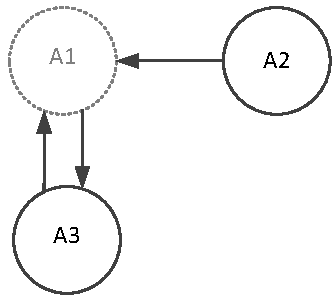
\includegraphics[width=\columnwidth]{img/Fig1}
\caption{Argumentation framework}
\label{fig:pras:example}
\end{figure}

Given an argumentation framework, the acceptability of arguments can be determined according to the appropriate argumentation semantics. The intuition is that an argument is acceptable if it is \emph{undefeated}, that is, any argument that attacks it, is itself defeated. Take, for example, the argumentation framework in Figure~\ref{fig:pras:example}. Argument A2 is undefeated because it has no attackers. This makes A1 defeated, because one of its attackers, A2, is undefeated. A3 is then also undefeated, since its only attacker, A1, is defeated by A2. Thus, the set of undefeated (justified) arguments given the argumentation framework in Figure~\ref{fig:pras:example} is $\{$A2, A3$\}$. 

In some cases, it is more difficult to determine whether or not an argument is defeated. Take, for example, the argumentation framework with just A1 and A3: they attack each other, they are alternatives and without any explicit preference, it is impossible to choose between the two. It is, however, possible to include explicit preferences between arguments when determining argument acceptability \cite{amgoud2002reasoning}. Take, for example, A1 and A3. If we say that we prefer the goal ``XXX'' (A1) over the goal ``YYY'' (A3), we remove the attack from A3 to A1 (Figure~\ref{fig:pras:example2}, left). This makes A1 the only undefeated argument, whereas A3 is now defeated. It is also possible to give explicit arguments for preferences \cite{modgil2009}. These arguments are then essentially attacks on attacks. For example, say we prefer A1 over A3 because ``XXX''. This can be rendered as a separate argument that attacks the attack from A3 to A1 (Figure~\ref{fig:pras:example2}, right), removing this attack and making $\{$A1, A4$\}$ the undefeated justified set of arguments.

\begin{figure}[ht]
\centering
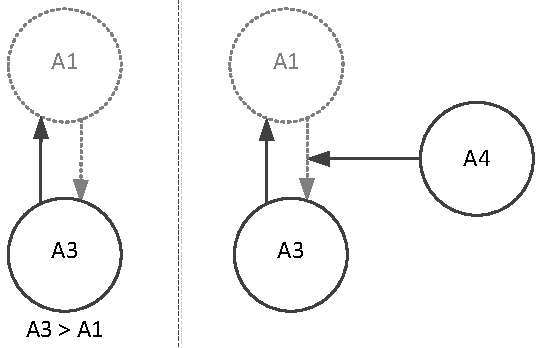
\includegraphics[width=\columnwidth]{img/Fig2}
\caption{Preferences between arguments}
\label{fig:pras:example2}
\end{figure}  

\subsubsection{Practical Reasoning and Goal Modeling}
\label{sect:background:pras:motivation}

Practical reasoning in the PRAS framework as described above provides a formally sound framework for defeasible reasoning about goals and actions that adheres to the acceptability semantics of Dung~\cite{Dung95} and its various extensions \cite{amgoud2002reasoning, modgil2009}. The usefulness of PRAS for the analysis of practical reasoning situations has been shown in different areas such as e-democracy~\cite{cartwright2009IS}, law~\cite{atkinson2005legal}, planning \cite{medellin2013planning} and choosing between safety critical actions \cite{tolchinsky2012deliberation}. The question in this paper is how PRAS can be adopted for use in goal modeling, so that we can capture the discussions between stakeholders that build a goal model as formal argumentation, thus adding a new evaluation technique for goal models that allows us to assess the \emph{acceptability} of elements of a goal model (as opposed to the \emph{satisfiability} \cite{}). 

PRAS (actions, goals, values) and GRL (tasks, goals, softgoals) have some obvious similarities, and in previous work \cite{vanzee-etal:renext2015,vanZee-etal:er2016} we already presented arguments based on PRAS of the form ``G is a goal, Action A realizes G \emph{Therefore} perform action A'' (see Figure~\ref{fig:pras:example3}, left, where the arrow denotes an inference step). These arguments, which can be constructed using the online OVA tool\footnote{\url{http://ova.arg-tech.org/}}, can be combined with further arguments providing, for example, expert opinions about the practical reasoning elements (Figure~\ref{fig:pras:example3}, right).

\begin{figure}[ht]
\centering
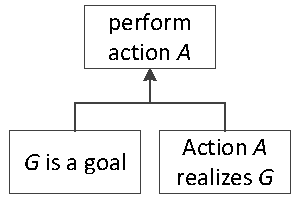
\includegraphics[width=\columnwidth]{img/Fig3}
\caption{Structured argument based on PRAS}
\label{fig:pras:example3}
\end{figure}  

The arguments built in OVA can automatically be translated to GRL diagrams using further online tooling\footnote{\url{https://github.com/RationalArchitecture/RationalGRL}}. This translation takes the elements of the arguments and directly translates this to GRL elements - any elements of arguments that have nothing to do with goal modelling (e.g. the expert opinion premise in Figure~\ref{fig:pras:example3}, right) can be included in the GRL diagram as \emph{beliefs}. 


For example, ... A similar approach, albeit without the explicit focus on practical reasoning, was taken by Jureta et al.~\cite{}, in which it translates similar structured arguments to goal diagrams. One of the problems of these approaches is that ...

The concept that appears in PRAS and not in GRL is \emph{circumstance}. In PRAS, an action $a$ is performed in current circumstances $R$, and by performing this action new circumstances $S$ are obtained. From this new circumstance $S$, another action may be performed again, and so on. In the AI literature, this type of reasoning usually referred to as ``AI planning''~\cite{weld1999recent}: from some initial state, find a sequence of actions such that a goal state is reached if these actions are executed. This planning approach is taken by a number of contributions using PRAS to create joint plans for a group of actors, often using a transition system as the underlying semantics~\cite{medellin2014}. However, in the early RE phase of an IS, one generally does not consider temporal planning. Decisions about the temporal order in which tasks should be executed are generally postponed until a later stage. In other words, goal modeling is not concerned with making plans, scenarios, or business processes for the information system. In URN (see section~\ref{sect:background:grl}) the distinction between goal modeling and business process modeling is clearly visible in the distinction between two separate modeling languages for the two activities. First, goal models are created in GRL and then, the use case maps (similar to business processes) are created in UCM. Therefore, when extending PRAS for GRL, we do not consider the notion of \emph{circumstances}.

The concept that appears in GRL but not in PRAS is \emph{resource}. A resource may be used by part of the system, or an actor, in order to perform a task or to reach a goal. Therefore, PRAS has to be extended with the notion of a resource in order for it to be applicable to GRL. %SGNew: to be applicable? don't understand the sentence. 

Finally, there are two concepts which appear in both models under different names. Where PRAS uses the notions ``action'' and ``value'', GRL uses the concepts ``task'' and respectively ``softgoal''. However, these two concepts are semantically identical.

With respect to relationships between concepts, the argument scheme PRAS from Section~\ref{sect:background:pras} contains the following relationships:\\

\noindent
R1. Actor $AG$ \emph{performs} action $A$\\
R2. Action $A$ \emph{realizes} goal $G$\\
R3. Goal $G$ \emph{promotes} value $S$\\
R4. Actor $AG$ \emph{has} goal $G$\\
R5. Actor $AG$ \emph{has} value $S$\\

\noindent

Relationships R4 and R5 are implicit in PRAS, but follow directly from its formulation (see~\cite{atkinson2007} for more details). The relationship ``promotes'' does not exist in GRL, but the relationship ``contributes to'' does, which is conceptually very similar. Therefore, we choose to use this relationship to formalize ``promotes'' relation.

As mentioned in Section~\ref{sect:background:grl}, GRL is a very non-restrictive modeling language, allowing intentional elements and links to be combined freely. Thus, GRL allows any links between any type of intentional element. PRAS, in contrast, only considers relationship R1-R5 above. As a result, the critical questions of PRAS are only applicable to a subset of all possible relationships in GRL. This, however, does not mean it is not possible to construct arguments and formulate critical questions for other relationship. In section~\ref{sect:implementation:implementation}, where we discuss the implementation of our tool, we explain in more detail that a user can straightforwardly add additional critical questions for other relationships as well.